\documentclass[noinstructornotes]{ximera}
%handout:  for handout version with no solutions or instructor notes
%handout,instructornotes:  for instructor version with just problems and notes, no solutions
%noinstructornotes:  shows only problem and solutions

%% handout
%% space
%% newpage
%% numbers
%% nooutcomes

%I added the commands here so that I would't have to keep looking them up
%\newcommand{\RR}{\mathbb R}
%\renewcommand{\d}{\,d}
%\newcommand{\dd}[2][]{\frac{d #1}{d #2}}
%\renewcommand{\l}{\ell}
%\newcommand{\ddx}{\frac{d}{dx}}
%\everymath{\displaystyle}
%\newcommand{\dfn}{\textbf}
%\newcommand{\eval}[1]{\bigg[ #1 \bigg]}

%\begin{image}
%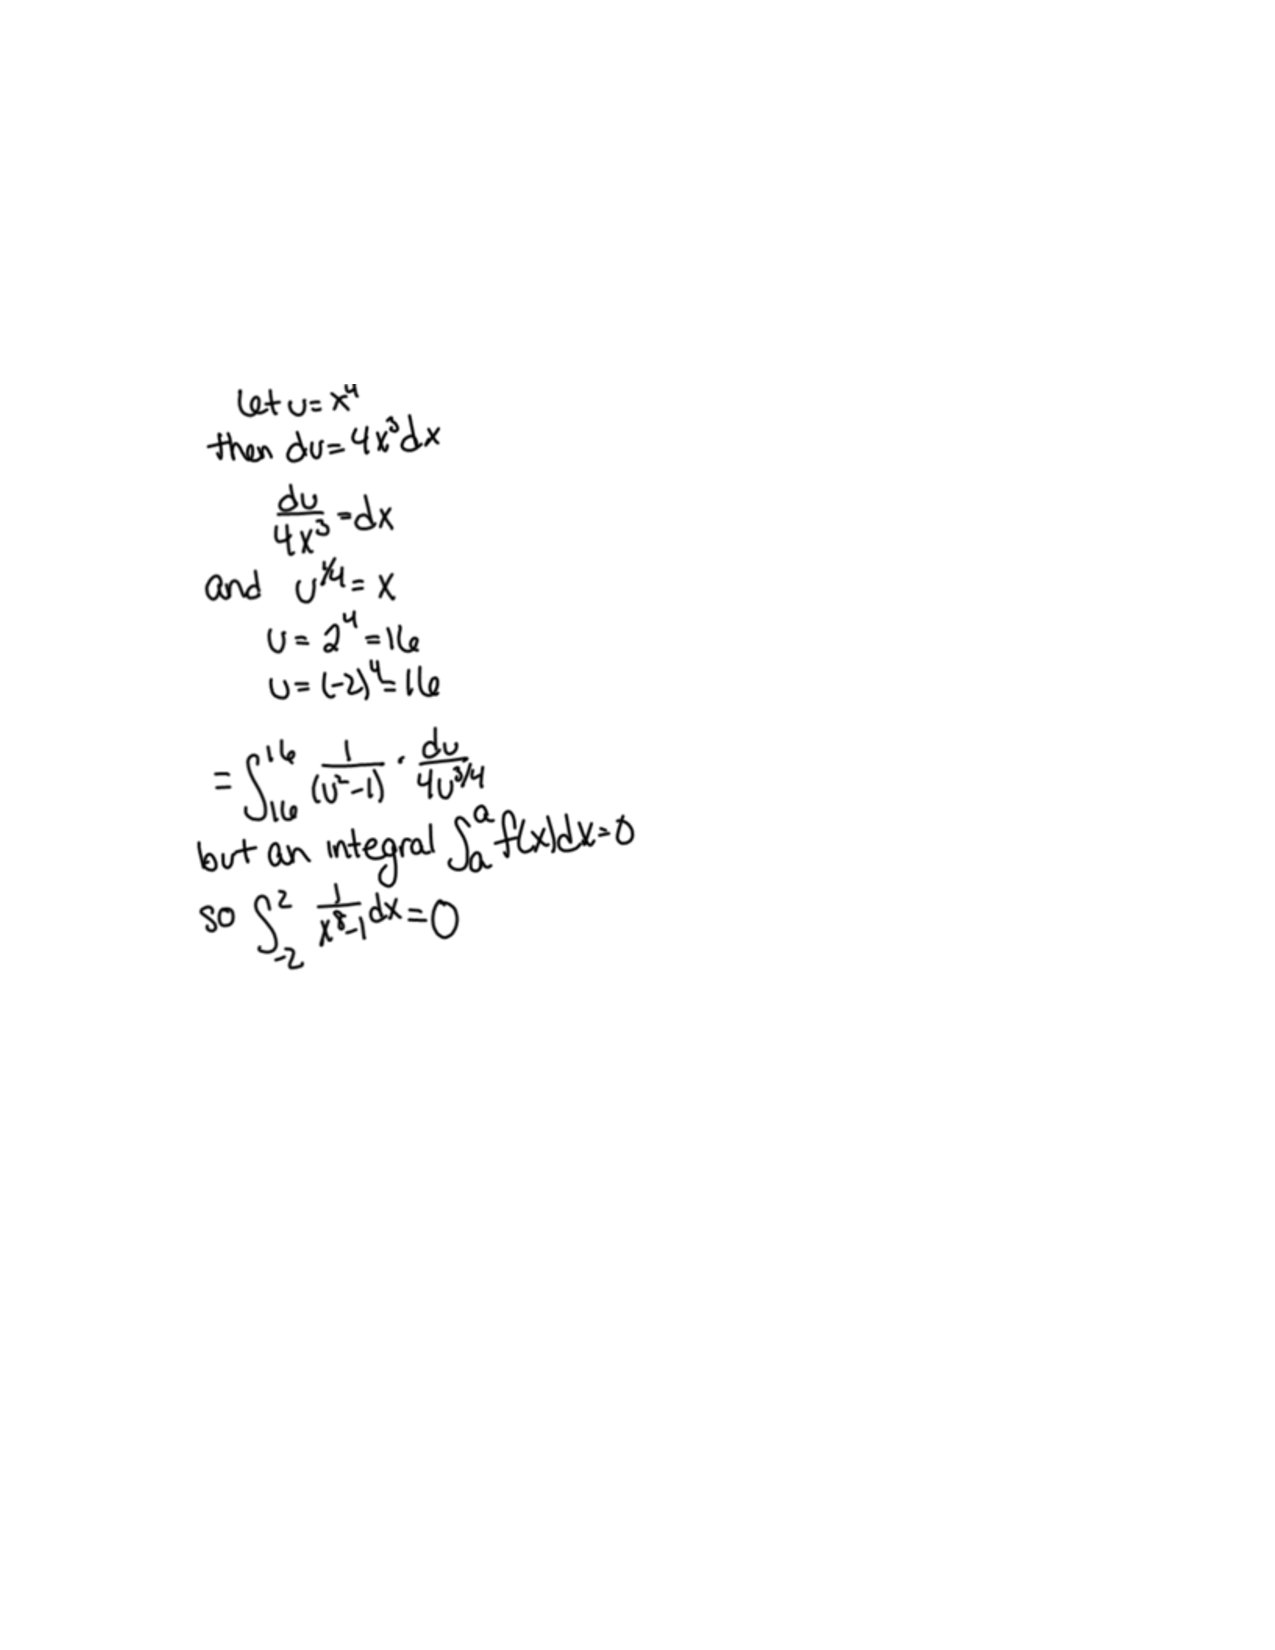
\includegraphics[trim= 170 420 250 180]{Figure1.pdf}
%\end{image}

%add a ``.'' below when used in a specific directory.
\newcommand{\RR}{\mathbb R}
\renewcommand{\d}{\,d}
\newcommand{\dd}[2][]{\frac{d #1}{d #2}}
\renewcommand{\l}{\ell}
\newcommand{\ddx}{\frac{d}{dx}}
\newcommand{\dfn}{\textbf}
\newcommand{\eval}[1]{\bigg[ #1 \bigg]}

\usepackage{multicol}

\renewenvironment{freeResponse}{
\ifhandout\setbox0\vbox\bgroup\else
\begin{trivlist}\item[\hskip \labelsep\bfseries Solution:\hspace{2ex}]
\fi}
{\ifhandout\egroup\else
\end{trivlist}
\fi} %% we can turn off input when making a master document

%\usepackage{fullpage}

\title{Section 7.8: Improper Integrals}  

\begin{document}
\begin{abstract}		\end{abstract}
\maketitle




\section{Warm up:}
%\begin{problem}
True or False:  It is possible for a region to be infinitely long but have a finite area.
	\begin{freeResponse}
	True.  Consider the region below the curve $y=\frac{1}{x^2}$, $x \geq 1$.
	\end{freeResponse}
	
\begin{instructorNotes}

\end{instructorNotes}
%\end{problem}





\section{Group work:}


% Problem 1
\begin{problem}
Review of limits:
	\begin{enumerate}
	
	\item  $\lim_{x \to -\infty} \left( 3x^{-6} + e^{5x} + \frac{\sin x}{x^2 + 3} \right)$
	\begin{freeResponse}
	Recall that the limit of a sum is the sum of the limits, provided that those limits exist.
		\begin{itemize}
		\item  $\lim_{x \to -\infty} 3x^{-6} = \lim_{x \to -\infty} \frac{3}{x^6} = 0$.
		\item  $\lim_{x \to -\infty} e^{5x} = 0$.
		\item  $\lim_{x \to -\infty} \frac{\sin x}{x^2 + 3} = 0$  
		
		\vspace{8pt}
		
		{\color{red} \text{To rigorously prove this, you need to use the squeeze theorem.}}
		\end{itemize}
	Thus, 
		\[
		\lim_{x \to -\infty} \left( 3x^{-6} + e^{5x} + \frac{\sin x}{x^2 + 3} \right) = 0
		\]
	\end{freeResponse}
	
	
	
	\item  $\lim_{x \to \infty} \frac{x}{\sqrt{9x^2+4}}$
	\begin{freeResponse}
		\begin{align*}
		\lim_{x \to \infty} \frac{x}{\sqrt{9x^2+4}}
		&= \lim_{x \to \infty} \frac{x}{\sqrt{x^2} \cdot {\sqrt{9 + \frac{4}{x^2}}}}  \\
		&= \lim_{x \to \infty} \frac{x}{|x| \cdot \sqrt{9 + \frac{4}{x^2}}}  \\
		&= \lim_{x \to \infty} \frac{x}{x \cdot \sqrt{9 + \frac{4}{x^2}}}  \\
		&= \lim_{x \to \infty} \frac{1}{\sqrt{9 + \frac{4}{x^2}}}  \\
		&= \frac{1}{\sqrt{9 + 0}} = \frac{1}{3}.
		\end{align*}
	\end{freeResponse}
	
	
	
	\item  $\lim_{x \to -\infty} \arctan x$
	\begin{freeResponse}
	$\lim_{x \to -\infty} \arctan x = - \frac{\pi}{2}. $
	\end{freeResponse}
	
	\end{enumerate}
		
\end{problem}

\begin{instructorNotes}
Review of limits.
\end{instructorNotes}








%problem 2
\begin{problem}
Determine if the given integral converges or diverges.  
If it converges, find the value.
	\begin{equation*}
	 \int_{-1}^{\infty} \frac{3}{2x+1} \d x
	\end{equation*}
	\begin{freeResponse}
	The function $\frac{3}{2x+1}$ has a vertical asymptote at $x=- \frac{1}{2}$.  
	So we rewrite the original integral as
		\[
		\int_{-1}^{\infty} \frac{3}{2x+1} \d x = \lim_{a \to -\frac{1}{2}^-} \int_{-1}^a \frac{3}{2x+1} \d x  
		+ \lim_{b \to -\frac{1}{2}^+} \int_b^0 \frac{3}{2x+1} \d x + \lim_{c \to \infty} \int_0^c \frac{3}{2x+1} \d x.
		\]
	The latter integral does not exist.  
	To see this, just note that
		\begin{align*}
		 \lim_{c \to \infty} \int_0^c \frac{3}{2x+1} \d x 
		 &= \lim_{c \to \infty} \eval{\frac{3}{2} \ln|2x+1|}_0^c  \\
		 &= \lim_{c \to \infty} \frac{3}{2} \ln|2c+1| = \infty.
		\end{align*}
	Therefore, 
		\[
		\int_{-1}^{\infty} \frac{3}{2x+1} \d x \; \text{ diverges.}
		\]
	\end{freeResponse}

	
%	\item  $\int_{-\infty}^{\infty} x e^{-x} \d x$
%	\begin{freeResponse}
%	\[
%	\int_{-\infty}^{\infty} x e^{-x} \d x = \lim_{a \to -\infty} \int_a^0 xe^{-x} \d x + \lim_{b \to \infty} \int_0^b xe^{-x} \d x.
%	\]
%	The first of these integrals does not exist.  
%	To see this, we apply integration by parts
%		\begin{align*}
%		\lim_{a \to -\infty} \int_a^0 xe^{-x} \d x
%		&= \lim_{a \to -\infty} \left( \eval{-xe^{-x}}_a^0 + \int_a^0 e^{-x} \d x \right)  \\
%		&= \lim_{a \to -\infty} \left( \left[ 0 + ae^{-a} \right] + \eval{-e^{-x}}_a^0 \right)  \\
%		&= \lim_{a \to -\infty} \left( ae^{-a} + e^{-a} - 1 \right)  \\
%		&= \lim_{a \to -\infty} \left( e^{-a}(a+1) - 1 \right)  \\
%		&= - \infty.
%		\end{align*}
%	Thus
%		\[
%		\int_{-\infty}^{\infty} x e^{-x} \d x \; \text{ diverges.}
%		\]
%	\end{freeResponse}
%	
%	
%	
%	\item  $\int_6^{\infty} \frac{2-4x}{2x^2 - 13x + 20} \d x$
%	\begin{freeResponse}
%	First notice that we can factor the denominator as
%		\[
%		2x^2 - 13x + 20 = (2x-5)(x-4).
%		\]
%	So we find a partial fraction decomposition of the integrand
%		\begin{align*}
%		&\frac{2-4x}{(2x-5)(x-4)} = \frac{A}{2x-5} + \frac{B}{x-4}  \\
%		\Longrightarrow \qquad &2-4x = A(x-4) + B(2x-5).
%		\end{align*}
%	We can solve for $A$ and $B$ via the following substitutions:
%		\begin{itemize}
%		\item {\color{red}$\left( \text{Let } x=\frac{5}{2} \right)$} \quad $2 - 4 \left(\frac{5}{2} \right) = A \left(\frac{5}{2} - 4 \right)$  \\
%			\[
%			-8 = - \frac{3}{2} A \qquad \Longrightarrow \qquad A = \frac{16}{3}.
%			\]
%		\item {\color{red} (Let $x=4$)}  \quad $2-16 = 3B \qquad \Longrightarrow \qquad B = - \frac{14}{3}$.
%		\end{itemize}
%	Thus, 
%		\begin{align*}
%		\int_6^{\infty} \frac{2-4x}{2x^2 - 13x + 20} \d x
%		&= \lim_{a \to \infty} \int_6^a \left[ \frac{\frac{16}{3}}{2x-5} - \frac{\frac{14}{3}}{x-4} \right] \d x  \\
%		&= \lim_{a \to \infty} \eval{ \frac{8}{3} \ln|2x-5| - \frac{14}{3} \ln|x-4| }_6^a  \\
%		&= \lim_{a \to \infty} \left[ \frac{8}{3} \left( \ln|2a-5| - \ln(7) \right) - \frac{14}{3} \left( \ln|a-4| - \ln(2) \right) \right]  \\
%		&= \lim_{a \to \infty} \left[ \frac{1}{3} \left( \ln(2a-5)^8 - \ln(a-4)^{14} \right) - \frac{8}{3} \ln (7) + \frac{14}{3} \ln(2) \right]  \\
%		&= \lim_{a \to \infty} \left[ \frac{1}{3} \ln \left( \frac{(2a-5)^8}{(a-4)^{14}} \right) - \frac{8}{3} \ln (7) + \frac{14}{3} \ln(2) \right]  \\
%		&= - \infty.
%		\end{align*}
%	Thus,
%		\[
%		\int_6^{\infty} \frac{2-4x}{2x^2 - 13x + 20} \d x \; \text{ diverges.}
%		\]
%	\end{freeResponse}
	
	
\end{problem}

\begin{instructorNotes}
Make sure that students write in the limit notation throughout their work, with the limit taken after the definite integral has been evaluated.
	\begin{enumerate}
	\item has a vertical asymptote as well as a limit going to infinity.
	\item is by parts, and L'Hospital's Rule will be useful for the limit.
	\item will need partial fractions.  
	The coefficients of the decomposition are rigged to be opposites of each other, so that one can use properties of logarithms to aid in taking the limit.
	\end{enumerate}
\end{instructorNotes}







%%problem 
%\begin{problem}
%Find the volume of the solid whose base is the region where $x \geq 1$, $y \geq 0$, and below the curve $y=\frac{1}{x^4}$, and whose cross sections perpendicular to the $x$-axis are squares.
%	\begin{freeResponse}
%	The area of each cross-section is $\left( \frac{1}{x^4} \right)^2 = \frac{1}{x^8}$.  
%	Thus,
%		\begin{align*}
%		{\color{red}\text{Volume }} &= \int_1^{\infty} \frac{1}{x^8} \d x  \\
%		&= \lim_{a \to \infty} \eval{- \frac{1}{7 x^7}}_1^a  \\
%		&= \lim_{a \to \infty} \left( - \frac{1}{7a^7} + \frac{1}{7} \right)  \\
%		&= 0 + \frac{1}{7} = \frac{1}{7}.
%		\end{align*}
%	\end{freeResponse}
%
%\end{problem}
%
%\begin{instructorNotes}
%
%\end{instructorNotes}




%
%%problem 2
%\begin{problem}
%Verify that, if $y(0)=0$, that both $f(x)=1-(x^2+1)^2$ \dfn{and} $g(x) = 1 - (x^2-1)^2$ are solutions to the differential equation $\dd[y]{x} = 4x\sqrt{1-y}$.
%	\begin{freeResponse}
%		\begin{align*}
%		f'(x) &= -2(x^2+1) \cdot 2x  \\
%		&= -4x \sqrt{(x^2+1)^2}  \\
%		&= -4x \sqrt{1-1+(x^2+1)^2}  \\
%		&= -4x \sqrt{1 - \left[1-(x^2+1)^2 \right]}  \\
%		&= -4x \sqrt{1-f(x)}.
%		\end{align*}
%		
%		\vskip 5pt
%		
%		\begin{align*}
%		g'(x) &= -2(x^2-1) \cdot 2x  \\
%		&= -4x \sqrt{(x^2-1)^2}  \\
%		&= -4x \sqrt{1-1+(x^2-1)^2}  \\
%		&= -4x \sqrt{1 - \left[1-(x^2-1)^2 \right]}  \\
%		&= -4x \sqrt{1-g(x)}.
%		\end{align*}
%	\end{freeResponse}
%		
%\end{problem}
%
%\begin{instructorNotes}
%Note that students will need to plug into both $x$ and $y$ in the differential equation.  
%Also, make sure that students realize that an initial value problem can possibly have many solutions.
%\end{instructorNotes}


%problem 1
\begin{problem}
	\begin{enumerate}
	\item  Show that 
		\begin{equation*}
		\frac{9}{2x^2+3x} = \frac{3}{x} - \frac{6}{2x+3}
		\end{equation*}
	
	\item  Determine if the integral
		\begin{equation*}
		\int_1^\infty \frac{9}{2x^2+3x} \d x
		\end{equation*}
	converges or diverges.  If it converges, give the value that it converges to.
	
	
	
	\begin{freeResponse}
	\begin{enumerate}
	\item
	Since $2x^2+3x = x(2x+3)$, we apply the method of partial fractions:
		\begin{align*}
		&\frac{9}{2x^2+3x} = \frac{A}{x} + \frac{B}{2x+3}  \\
		\Longrightarrow \qquad &9 = A(2x+3) + Bx.
		\end{align*}
	Letting $x=0$ gives that
		\begin{equation*}
		9 = 3A	\quad	\Longrightarrow \quad	A = 3.
		\end{equation*}
	Then letting $x = -\frac{3}{2}$, we see that
		\begin{equation*}
		9 = - \frac{3}{2} B \quad \Longrightarrow \quad B = - 9 \cdot \frac{2}{3} = -6.
		\end{equation*}
	Therefore, plugging in our values for $A$ and $B$ gives us
		\begin{equation*}
		\frac{9}{2x^2+3x} = \frac{3}{x} - \frac{6}{2x+3}.
		\end{equation*}
		
		
		
	\item We have that
		\begin{align*}
		\int_1^\infty \frac{9}{2x^2+3x} \d x &= \lim_{t \to \infty} \int_1^t \left( \frac{3}{x} - \frac{6}{2x+3} \right) \d x  \\
		&= \lim_{t \to \infty} \eval{3\ln|x| - \frac{6}{2} \ln|2x+3|}_1^t  \quad {\color{red}\text{don't forget to divide the 6 by 2}}  \\
		&= \lim_{t \to \infty} \left( 3\ln|t| - 3\ln|2t+3| - 0 + 3\ln(5) \right)  \quad {\color{red}\ln(1) = 0} \\
		&= \lim_{t \to \infty} \left( 3 \ln \left| \frac{5t}{2t+3} \right| \right)  \quad {\color{red}\text{properties of logarithms}}  \\
		&= \boxed{3 \ln \left( \frac{5}{2} \right)}	\quad	{\color{red}\text{since ln(x) is a continuous function}}
		\end{align*}
	
	\end{enumerate}
	\end{freeResponse}
	
	\end{enumerate}
	
		
\end{problem}












%problem 2
\begin{problem}
		\begin{enumerate}
	\item  Show that 
		\begin{equation*}
		\frac{6x-8}{x^3+4x} = \frac{2x+6}{x^2+4} - \frac{2}{x}
		\end{equation*}
	
	\item  Determine if the integral
		\begin{equation*}
		\int_3^\infty \frac{6x-8}{x^3+4x} \d x
		\end{equation*}
	converges or diverges.  If it converges, give the value that it converges to.
	
	
	
	\begin{freeResponse}
	\begin{enumerate}
	\item
	Since $x^3+4x = x(x^2+4)$, we use partial fractions:
		\begin{align*}
		&\frac{6x-8}{x^3+4x} = \frac{Ax+B}{x^2+4} + \frac{C}{x}  \\
		\Longrightarrow 	\qquad	&6x-8 = (Ax+B)(x) + C(x^2+4).
		\end{align*}
	Letting $x=0$, we see that
		\begin{equation*}
		-8 = 4C \quad \Longrightarrow \quad C = -2.
		\end{equation*}
	To find $A$ and $B$, let us plug in $C=-2$ and simplify:
		\begin{align*}
		6x-8 &= Ax^2 + Bx -2x^2 - 8  \\
		&= (A-2)x^2 + Bx - 8.
		\end{align*}
	Aligning the respective coefficients, we see that
		\begin{align*}
		&A-2 = 0	\quad	\text{and}	\quad	B=6  \\
		\Longrightarrow		\quad	&A=2	\quad	\text{and}	\quad	B=6.
		\end{align*}
	Finally, plugging this into the original equation yields
		\begin{equation*}
		\frac{6x-8}{x^3+4x} = \frac{2x+6}{x^2+4} - \frac{2}{x}.
		\end{equation*}
		
		
		
		
	\item We have that
		\begin{align*}
		\int_3^\infty \frac{6x-8}{x^3+4x} \d x &= \lim_{t \to \infty} \int_3^t \left( \frac{2x+6}{x^2+4} - \frac{2}{x} \right) \d x  \\
		&= \lim_{t \to \infty} \left( \int_3^t \frac{2x}{x^2+4} \d x + \int_3^t \frac{6}{x^2+4} \d x - \int_3^t \frac{2}{x} \d x \right).
		\end{align*}
	Let us evaluate each integral separately, combine them, and then take the limit.
	
		\begin{enumerate}
		\item[(i)]  \begin{align*}
		\int_3^t \frac{2x}{x^2+4} \d x &= \int_{13}^{t^2+4} \frac{1}{w} \d w	\quad	{\color{red}w=x^2+4, \d w = 2x \d x}  \\
		&= \ln(t^2 +4) - \ln(13).
		\end{align*}
		
		\item[(ii)]  \begin{align*}
		\int_3^t \frac{6}{x^2+4} \d x &= \eval{\frac{6}{2} \arctan \left( \frac{x}{2} \right) }_3^t  \\
		&= 3 \arctan \left(\frac{t}{2} \right) - 3 \arctan \left( \frac{3}{2} \right).
		\end{align*}
		
		\item[(iii)]  \begin{align*}
		\int_3^t \frac{2}{x} \d x &= \eval{ 2 \ln|x| }_3^t  \\
		&= 2 \ln|t| - 2\ln(3).
		\end{align*}
		
		\end{enumerate}
	We now combined these three expressions, and then compute the limit.
		\begin{align*}
		&\int_3^\infty \frac{6x-8}{x^3+4x} \d x  \\
		&= \lim_{t \to \infty} \left[ \left(\ln(t^2 +4) - \ln(13) \right) + \left( 3 \arctan \left(\frac{t}{2} \right) - 3 \arctan \left( \frac{3}{2} \right) \right) - \left( 2 \ln|t| - 2\ln(3) \right) \right]  \\
		&= \lim_{t \to \infty} \left[ \ln(t^2+4) - \ln t^2 + 3 \arctan \left( \frac{t}{2} \right) - \ln 13 + \ln 9 - 3 \arctan \left( \frac{3}{2} \right) \right]  \\
		&= \lim_{t \to \infty} \left[ \ln \left( \frac{t^2+4}{t^2} \right) + 3 \arctan \left( \frac{t}{2} \right) - \ln 13 + \ln 9 - 3 \arctan \left( \frac{3}{2} \right) \right]  \\
		&= \ln(1) + 3 \cdot \frac{\pi}{2} - \ln 13 + \ln 9 - 3 \arctan \left( \frac{3}{2} \right) 	\quad	{\color{red}\lim_{t \to \infty} \arctan(t) = \frac{\pi}{2}}\\
		&= \boxed{\frac{3\pi}{2} - \ln 13 + \ln 9 - 3 \arctan \left( \frac{3}{2} \right)}	\quad	{\color{red}\text{if you like, }- \ln 13 + \ln 9 = \ln \left( \frac{9}{13} \right)}
		\end{align*}
	
	\end{enumerate}
	\end{freeResponse}
	
	\end{enumerate}
\end{problem}

\begin{problem}
Given that $\displaystyle \dfrac{37}{(2x-1)(x^2+9)} = \dfrac{4}{2x-1} - \dfrac{2x+1}{x^2+9}$, evaluate: $$\displaystyle \int_3^{\infty} \dfrac{37}{(2x-1)(x^2+9)} \, dx$$
 

\begin{freeResponse}\begin{align} 
 \displaystyle \int_3^{\infty} \dfrac{37}{(2x-1)(x^2+9)} \, dx &= \lim_{b \rightarrow \infty} \displaystyle \int_3^{b} \left(\dfrac{4}{2x-1} - \dfrac{2x+1}{x^2+9}\right) \, dx \nonumber \\
 &= \lim_{b \rightarrow \infty} \displaystyle \int_3^{b} \left(\dfrac{4}{2x-1} - \dfrac{2x}{x^2+9}- \dfrac{1}{x^2+9}\right) \, dx  \label{eq1}
 \end{align}
 
 We compute the antiderivatives of each term separately:
 
 \begin{itemize}
 \item For $\displaystyle \int \dfrac{4}{2x-1} \, dx$, let $u = 2x -1 \rightarrow du = 2 dx \rightarrow   dx = \dfrac{du}{2}$.
 
\hspace{5mm} Thus, $\displaystyle \int \dfrac{4}{2x-1} \, dx = \int \dfrac{4}{u} \left(\dfrac{du}{2}\right) = 2 \ln |u| + C = \underline{2 \, \ln |2x+1| +C}$
 
 \vspace{3mm}
 
  \item For $\displaystyle \int \dfrac{2x}{x^2+9} \, dx$, let $u = x^2+9 \rightarrow du = 2x dx \rightarrow   dx = \dfrac{du}{2x}$.
  
\hspace{5mm}
 Thus, $\displaystyle \int \dfrac{2x}{x^2+9} \, dx = \int \dfrac{2x}{u} \left(\dfrac{du}{2x}\right) =  \ln |u| + C = \underline{ \ln (x^2+9) +C}$
 
  \item For $\displaystyle \int \dfrac{1}{x^2+9} \, dx$, recall the important formula $\displaystyle \int \dfrac{1}{x^2+a^2} \, dx = \dfrac{1}{a} \arctan \dfrac{x}{a} +C$.
    
\hspace{5mm} Thus, $\displaystyle \int \dfrac{1}{x^2+9} \, dx = \underline{\dfrac{1}{3} \arctan \dfrac{x}{3} +C}$
 
 \end{itemize}

Substituting these results into (\ref{eq1}) and dropping the constants since this is a definite integral  gives:
\begin{align*}
\displaystyle \int_3^{\infty} \dfrac{37}{(2x-1)(x^2+9)} \, dx &= \lim_{b \rightarrow \infty} \left[2 \, \ln |2x-1|-\ln (x^2+9) -\dfrac{1}{3} \arctan \dfrac{x}{3} \right|_3^b\\
\end{align*}
 To evaluate the resulting limit correctly, you \emph{MUST} combine the logarithms:
 \begin{align*}
\displaystyle \int_3^{\infty} \dfrac{37}{(2x-1)(x^2+9)} \, dx &= \lim_{b \rightarrow \infty} \left[ \, \ln (2x-1)^2-\ln (x^2+9) -\dfrac{1}{3} \arctan \dfrac{x}{3} \right|_3^b\\
 &= \lim_{b \rightarrow \infty} \left[ \, \ln \left( \dfrac{4x^2-4x+1}{x^2+9}\right) -\dfrac{1}{3} \arctan \dfrac{x}{3} \right|_3^b\\
  &= \lim_{b \rightarrow \infty} \, \left[ \left\{ \ln \left( \dfrac{4b^2-4b+1}{b^2+9} \right)-\dfrac{1}{3} \arctan \dfrac{b}{3} \right\} -\left\{\ln \left( \dfrac{25}{18} \right) -\dfrac{1}{3} \arctan 1 \right\} \right]\\
  &=  \ln \left[\lim_{b \rightarrow \infty} \, \dfrac{4b^2-4b+1}{b^2+9} \right]-\dfrac{1}{3}  \ln \left[\lim_{b \rightarrow \infty} \, \arctan \dfrac{b}{3} \right]- \ln \left( \dfrac{25}{18}\right) +\dfrac{1}{3}  \cdot \dfrac{\pi}{4} \\
  &=  \ln 4-\dfrac{1}{3} \cdot \dfrac{\pi}{2} - \ln \left( \dfrac{5}{18} \right) +\dfrac{\pi}{12} \\
    &= \boxed{\ln \left( \dfrac{72}{25} \right)-\dfrac{\pi}{12} }\\
\end{align*}

\end{freeResponse}
\end{problem}























	
	
	
	
	
	
	
	
	

	










								
				
				
	







	
	
	
	
	
	
	
	
	

	










								
				
				
	














\end{document} 


















